  \paragraph\
      Cassandra C client is a wrapper around Cassandra Python client that is Pycassa. I used C-Python API
      to write wrapper around Python's Pycassa API. 
  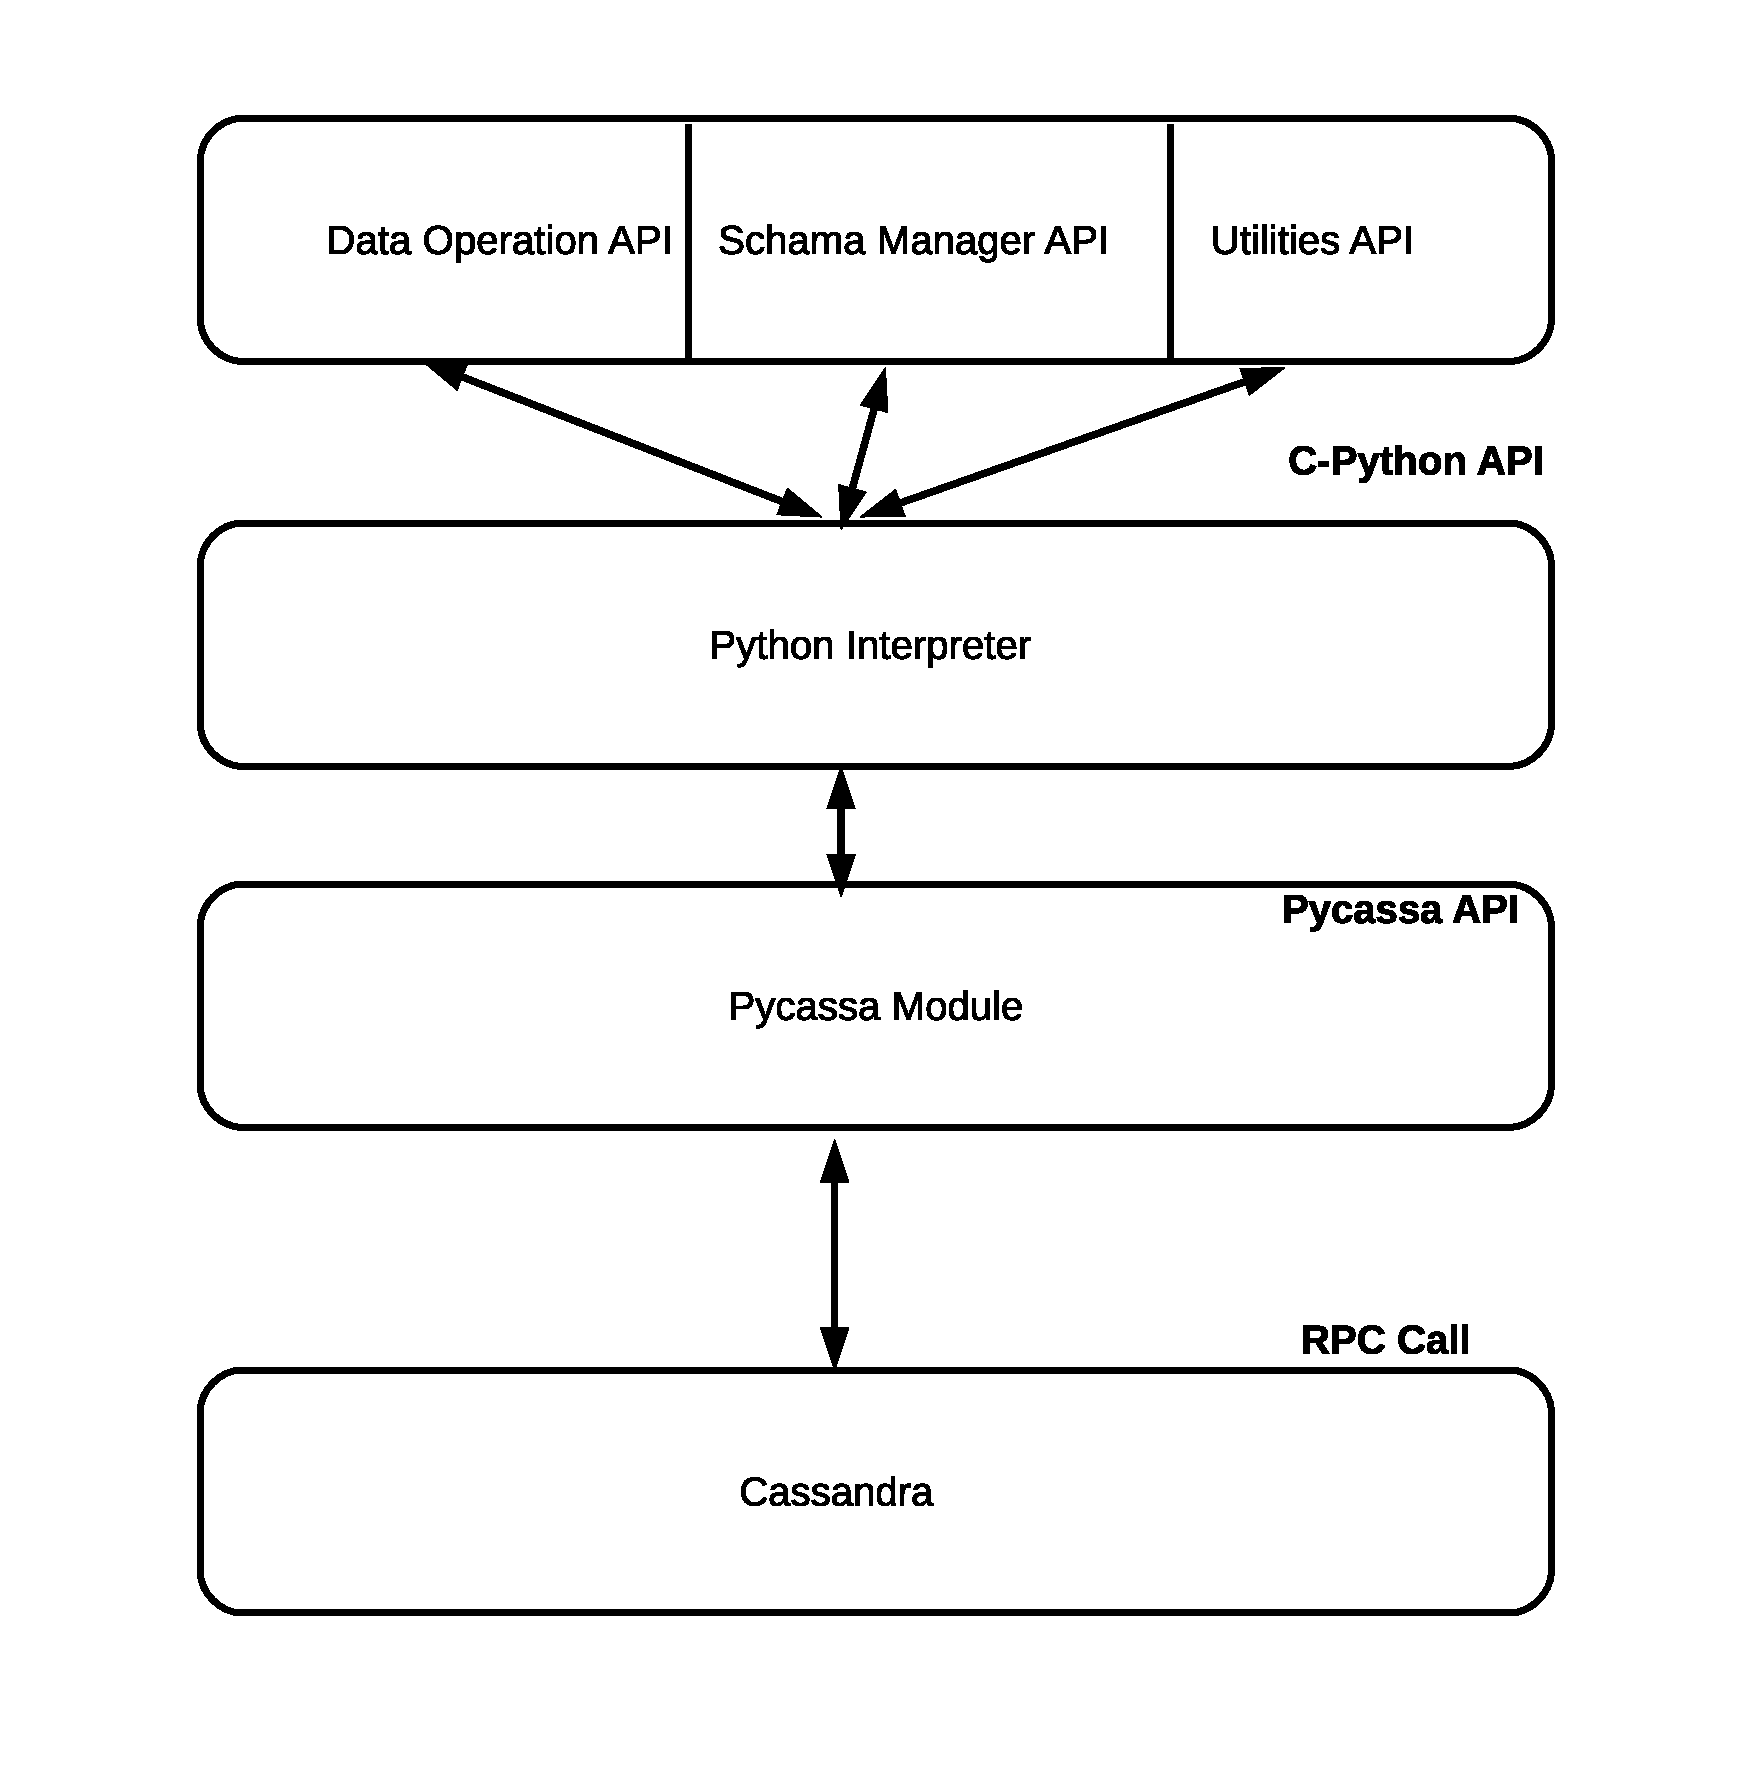
\includegraphics[scale=0.3]{C_client.eps}

 
\subsection{API Clasification} 

%%%%%%%%%%%%%%%%%%%%%%%%%%%%%%%%%%%%%%%%%%%%%%%%%%%%%%%%%%%%%%%%%%%%%%%%%%%%

\subsection{Utilities APIs} 

%%%%%%%%%%%%%%%%%%%%%%%%%%%%%%%%%%%%%%%%%%%%%%%%%%%%%%%%%%%%%%%%%%%%%%%%%%%%


 \begin{tabular}{p{7cm}}
  {\bf Utilities APIs } \\
  
\begin{enumerate}
   \item isExistPycassa()
   \item isExistKeyspace()
   \item isExistColumnfamily()

   \end{enumerate} 
 \end{tabular}
%%%%%%%%%%%%%%%%%%%%%%%%%%%%%%%%%%%%%%%%%%%%%%%%%%%%%%%%%%%%%%%%%%%%%%%%%%%
\subsubsection{isExistPycassa()}
\begin{verbatim}
int isExistPycassa(void);
\end{verbatim}

  It checks whether pycassa is installed or not in the system.

  \paragraph{Arguments:} Void.

 \paragraph{Return Value:}
 It returns a Boolean to indicate status.
\begin{enumerate}
 \item If Exist : 1.
 \item If Not Exist   : 0.
\end{enumerate}
%%%%%%%%%%%%%%%%%%%%%%%%%%%%%%%%%%%%%%%%%%%%%%%%%%%%%%%%%%%%%%%%%%%%%%%%%%%%


\subsubsection{isExistKeyspace()}
\begin{verbatim}
int isExistKeyspace(char *keyspace, char *server);
\end{verbatim}

  It checks existence of keyspace on the Cassandra server.

  \paragraph{Arguments:} 
	        \begin{enumerate}
		    \item keyspace: Name of the keyspace.
		    \item server : IP address and port number of server \{ex 127.0.0.1:9160\}.
		\end{enumerate}
		
 \paragraph{Return Value:}
 It returns a Boolean to indicate status.
\begin{enumerate}
 \item If Exist : 1.
 \item If Not Exist   : 0.
\end{enumerate}
%%%%%%%%%%%%%%%%%%%%%%%%%%%%%%%%%%%%%%%%%%%%%%%%%%%%%%%%%%%%%%%%%%%%%%%%%%%%

\subsubsection{isExistColumnfamily()}
\begin{verbatim}
int isExistColumnfamily(char *keyspace, char *columnfamily, char *server);
\end{verbatim}

   It checks existence of column family in a specified keyspace on the Cassandra server.

  \paragraph{Arguments:} 
	        \begin{enumerate}
		    \item keyspace: Name of the keyspace.
		    \item column family: Name of the column family.
		    \item server : IP address and port number of server \{ex 127.0.0.1:9160\}.
		\end{enumerate}
		
 \paragraph{Return Value:}
 It returns a Boolean to indicate status.
\begin{enumerate}
 \item If Exist : 1.
 \item If Not Exist   : 0.
\end{enumerate}
%%%%%%%%%%%%%%%%%%%%%%%%%%%%%%%%%%%%%%%%%%%%%%%%%%%%%%%%%%%%%%%%%%%%%%%%%%%%%%%%%%%%%%%%%%%%%%%%%%

%%%%%%%%%%%%%%%%%%%%%%%%%%%%%%%%%%%%%%%%%%%%%%%%%%%%%%%%%%%%%%%%%%%%%%%%%%%%%%%%%%%%%%%%%%%%%%%%%


\subsection{Schema Manager APIs} 

%%%%%%%%%%%%%%%%%%%%%%%%%%%%%%%%%%%%%%%%%%%%%%%%%%%%%%%%%%%%%%%%%%%%%%%%%%%%
\begin{tabular}{ p{7cm} }
 {\bf Schema Manager APIs}\\
  
\begin{enumerate}
   \item cassandraCreateKeyspace()
   \item cassandraCreateColumnFamily()
   \item cassandraDropColumnFamily()
   \item cassandraDropKeyspace()
   \end{enumerate} \\

\end{tabular}
\subsubsection{cassandraCreateKeyspace()}
\begin{verbatim}
 int cassandraCreateKeyspace(char *keyspace, char *strategy, int rf, 
                             char *server);
\end{verbatim}

  It creates keyspace with the specified name.

  \paragraph{Arguments}
  \begin{enumerate}
   \item keyspace: name of the keyspace.
   \item strategy : Replication strategy have to either of the followings as string
		    \begin{enumerate}
		     \item SimpleStrategy
		     \item NetworkTopologyStrategy
		     \item OldNetworkTopologyStrategy
		    \end{enumerate}

   \item rf:       Replication factor for the keyspace.
   \item server : IP address and port number of server \{ex 127.0.0.1:9160\}.
  \end{enumerate}

 \paragraph{Return Value:}
 It returns an integer for indicating success or failure.
\begin{enumerate}
 \item On Success : 0.
 \item On Error   : -1.
\end{enumerate}
%%%%%%%%%%%%%%%%%%%%%%%%%%%%%%%%%%%%%%%%%%%%%%%%%%%%%%%%%%%%%%%%%%%%%%%%%%%%

\subsubsection{cassandraCreateColumnFamily()}
\begin{verbatim}
 int cassandraCreateColumnFamily(char *keyspace, char *columnfamily,
                                 char *comparator, char *server);
\end{verbatim}

  It creates a column family with specified name and comparator.

  \paragraph{Arguments}
  \begin{enumerate}
   \item keyspace: Name of the keyspace.
   \item column family: Name of the column family to be created.
   \item comparator : For defining composite column family. Support following data types as string
		    \begin{enumerate}
		     \item AsciiType
		     \item DoubleType
		     \item IntegerType
		     \item BytesType
		     \item LongType
		     \item FloatType
		     \item TimeUUIDType
		    \end{enumerate}

   \item server : IP address and port number of server \{ex 127.0.0.1:9160\}.
  \end{enumerate}

 \paragraph{Return Value:}
 It returns an integer  for indicating success or failure.
\begin{enumerate}
 \item On Success : 0.
 \item On Error   : -1.
\end{enumerate}
\paragraph{Example:}
\begin{verbatim}
 cassandraCreateColumnFamily("testKeyspace", "testCF", "AsciiType IntegerType", 
                             "127.0.0.1:9160");
\end{verbatim}

%%%%%%%%%%%%%%%%%%%%%%%%%%%%%%%%%%%%%%%%%%%%%%%%%%%%%%%%%%%%%%%%%%%%%%%%%%%%

\subsubsection{cassandraDropColumnFamily()}
\begin{verbatim}
int cassandraDropColumnFamily(char *keyspace, char *columnfamily, char *server);
\end{verbatim}

  It drops  column family from specified keyspace.

  \paragraph{Arguments}
  \begin{enumerate}
   \item keyspace: Name of the keyspace.
   \item column family: Name of the column family to be deleted.
   \item server : IP address and port number of server \{ex 127.0.0.1:9160\}.
  \end{enumerate}

 \paragraph{Return Value:}
 It returns an integer  for indicating success or failure.
\begin{enumerate}
 \item On Success : 0.
 \item On Error   : -1.
\end{enumerate}
%%%%%%%%%%%%%%%%%%%%%%%%%%%%%%%%%%%%%%%%%%%%%%%%%%%%%%%%%%%%%%%%%%%%%%%%%%%%

\subsubsection{cassandraDropKeyspace()}
\begin{verbatim}
int cassandraDropKeyspace(char *keyspace, char *server);
\end{verbatim}

  It drops  keyspace from the server.

  \paragraph{Arguments}
  \begin{enumerate}
   \item keyspace: Name of the keyspace.
   \item server : IP address and port number of server \{ex 127.0.0.1:9160\}.
  \end{enumerate}

 \paragraph{Return Value:}
 It returns an integer  for indicating success or failure.
\begin{enumerate}
 \item On Success : 0.
 \item On Error   : -1.
\end{enumerate}
%%%%%%%%%%%%%%%%%%%%%%%%%%%%%%%%%%%%%%%%%%%%%%%%%%%%%%%%%%%%%%%%%%%%%%%%%%%%

\subsection{Data Operation APIs} 
\paragraph{}These APIs allows  manipulation of data in Cassandra.

\begin{tabular}{ p{7cm} }

    {\bf Data Operation APIs}     \\
 

\begin{enumerate}
\item cassandraConnect()
   \item cassandraInsert()
   \item cassandraGet()
   \item cassandraGetNext()
   \end{enumerate} 
\end{tabular}


%\begin{center}


%\end{center}



%%%%%%%%%%%%%%%%%%%%%%%%%%%%%%%%%%%%%%%%%%%%%%%%%%%%%%%%%%%%%%%%%%%%%%%%%%
\subsubsection{cassandraConnect()}
\begin{verbatim}
 int cassandraConnect(char *keyspace, char *columnfamily, char *server);
\end{verbatim}

  Connects to a Cassandra server to specific keyspace and column family.

  \paragraph{Arguments}
  \begin{enumerate}
   \item keyspace: Name of the keyspace to use.
   \item column family : Name of the column family in specified keyspace.
   \item server :       IP:port number of server \{ex 127.0.0.1:9160\}.
  \end{enumerate}

 \paragraph{Return Value:}
 It returns an integer that points to the column family for reading and writing operation.
\begin{enumerate}
 \item On Success : Non-Negative integer. 
 \item On Error   : -1.
\end{enumerate}
%%%%%%%%%%%%%%%%%%%%%%%%%%%%%%%%%%%%%%%%%%%%%%%%%%%%%%%%%%%%%%%%%%%%%%%%%%%

\subsubsection{cassandraInsert()}
\begin{verbatim}
 int cassandraInsert (int cfDesc, char *key, char *value, char *columnName, ...);
\end{verbatim}

  Insert  a key:value pair to the column family referred by cfDesc.

  \paragraph{Arguments}
  \begin{enumerate}
   \item cfDesc: Descriptor return by cassandraConnect().
   \item key : Name of row key .
   \item value :       Value of the column.
   \item columnName : A formated string for composite or simple column name.
  \end{enumerate}

 \paragraph{Return Value:}
 It returns an integer for indicating success or failure.
\begin{enumerate}
 \item On Success : 0.
 \item On Error   : -1.
\end{enumerate}
%%%%%%%%%%%%%%%%%%%%%%%%%%%%%%%%%%%%%%%%%%%%%%%%%%%%%%%%%%%%%%%%%%%%%%%%%%%%

\subsubsection{cassandraGet()}
\begin{verbatim}
 result_t * cassandraGet (int cfDesc, char *rowkey, char *colStart, 
                          char *colEnd, int colCount);
\end{verbatim}

  Insert  a key:value pair to the column family referred by cfDesc.

  \paragraph{Arguments}
  \begin{enumerate}
   \item cfDesc: Descriptor return by cassandraConnect().
   \item rowkey : Name of row key .
   \item colStart :  Name of the column to start fetching data.
   \item colEnd : Name of the column to stop fetching data.
   \item colCount: Number of columns to fetch.
  \end{enumerate}

 \paragraph{Return Value:}
 It returns a array of key-value pair.
  \begin{enumerate}
 \item On Success : result\_t *.
 \item On Error   : NULL.
\end{enumerate}
%%%%%%%%%%%%%%%%%%%%%%%%%%%%%%%%%%%%%%%%%%%%%%%%%%%%%%%%%%%%%%%%%%%%%%%%%%%%

\subsubsection{cassandraGetItem()}
\begin{verbatim}
 int cassandraGetItem( result_t *, int position, char *colName, 
                       char *colValue);
\end{verbatim}

  It fetch  a key:value pair by position.

  \paragraph{Arguments}
  \begin{enumerate}
   \item result\_t *: Result array return cassandraGet().
   \item key : Name of row key .
   \item position : Position of the element to be return. 
  \end{enumerate}
\paragraph{Output Arguments}
\begin{enumerate}
 \item colName: Name of the column.
 \item colValue: Value at the column.
\end{enumerate}

 \paragraph{Return Value:}
 It returns an integer  for indicating success or failure.
\begin{enumerate}
 \item On Success : 0.
 \item On Error   : -1.
\end{enumerate}
%%%%%%%%%%%%%%%%%%%%%%%%%%%%%%%%%%%%%%%%%%%%%%%%%%%%%%%%%%%%%%%%%%%%%%%%%%%%


%%%%%%%%%%%%%%%%%%%%%%%%%%%%%%%%%%%%%%%%%%%%%%%%%%%%%%%%%%%%%%%%%%%%%%%%%%%%

\section{Modifications Made on \emph{ntop} }

\subsection{\emph{ntop} Plugin Structure}
\emph{ntop} uses  shared objects technology to provide plug-in, 
that allows dynamic linking of compiled shared objects  to \emph{ntop} to add extra features. \\ \\

\textbf{\emph{ntop} support following API for plug-in support:}\\ \\
\begin{tabular}{|l|l|}
\hline
 \textbf{API name} &  \textbf{Details}\\
\hline
 int(*IntFunct)(void); & Called at initialization of the plug-in.\\
 \hline
 void(*VoidFunct)(u\_char); & Called at termination of the plug-in.\\
 \hline
 void(*PluginHTTPFunct)(char* url); & HTTP request handler function.\\
 \hline
\end{tabular}
\subsection{Changes Made}
\paragraph{Added files:}
\begin{enumerate}
 \item ntop/plugins/cassandraPlugin.c
 \item ntop/plugins/cassandraPlugin.h
\end{enumerate}
\paragraph{Modified files:}
\begin{enumerate}
 \item ntop/plugins/Makefile.am
 \item ntop/python.c
\end{enumerate}

\textbf{APIs for Cassandra Plug-in}\\

\begin{tabular}{|l|l|}
\hline
 \textbf{API name} &  \textbf{Details}\\
\hline
 int initCassandraFunct (void); & Initialize the plug-in.\\
 \hline
 void termCassandraFunct (u\_char termNtop); & Terminate the plug-in.\\
 \hline
 handlecassandraHTTPrequest (char *\_url); & Handle HTTP request.\\
 \hline
  void* cassandraMainLoop(void* notUsed \_UNUSED\_); & statistics collector thread;\\
  \hline
\end{tabular}

\subsection{CassandraPlugin Life Cycle}
          \begin{figure}[htb]
	    \centering
	    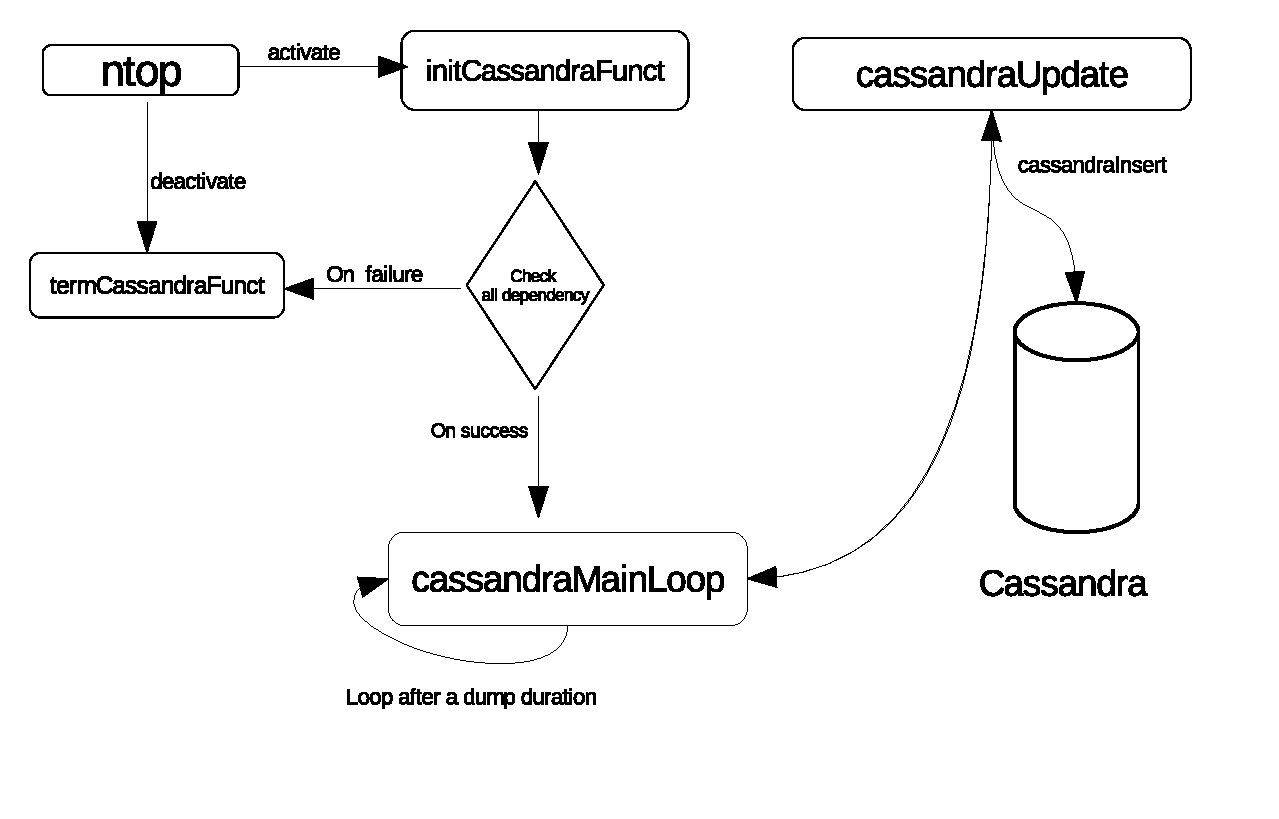
\includegraphics[scale = .5]{lfc.eps}
	    %\caption{Cassandra Performance\cite{cassathpt}.} 
	  \end{figure}


